\scanpage{44}
petits clous\\
\unsure{percer|pince|perceur|pour} \unsure{baguette|baguettes}\\
planchette

\figure{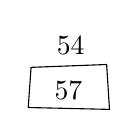
\begin{tikzpicture}[x=.6cm,y=.6cm]
\draw (0,0)--(.06,.85)--(1.66,.91)--(1.72,-.04)--(0,0);
\node[above] at (.9,.91) {$54$};
\node[above] at (.85,-.04) {$57$};
\end{tikzpicture}}
\figure{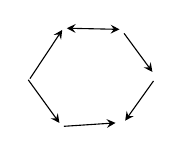
\begin{tikzpicture}[x=.72cm,y=.72cm,>=stealth]
\draw[->] (-1.1,0)--(-.53,.86); \draw[<->] (-.45,.89)--(.48,.87);
\draw[->] (.56,.8)--(1.06,.12); \draw[->] (1.08,-.04)--(.58,-.74);
\draw[->] (-.5,-.84)--(.41,-.78); \draw[->] (-1.13,-.02)--(-.58,-.78);
\end{tikzpicture}}
\figure{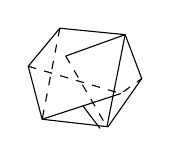
\begin{tikzpicture}[scale=.68]
\draw (-1.08,.27)--(-.49,.98)--(.73,.86)--(1.04,.04)--(.41,-.86)--(-.82,-.72)--cycle;
\draw (-.82,-.72)--(.65,-.24) (.73,.86)--(-.38,.46) (.73,.86)--(.39,-.86) (-.06,-.47)--(.26,-.89);
\draw[dashed] (-.49,.98)--(-.82,-.72) (-1.08,.27)--(.65,-.24)--(1.04,.04) (-.38,.46)--(.39,-.86);
\end{tikzpicture}}

\[
\begin{aligned}
 S&=\tau\times\varepsilon
 &\widetilde S&=\tau\times\varepsilon\times\omega(\tau)\\
 A&=\tau\times(\varepsilon\wedge\omega(\tau))
 &&\tau\times\varepsilon\mathbin{\cdot}\tau\times\varepsilon'\\
 &\tau\times(\varepsilon\wedge\omega(\tau))\wedge\omega(\unsure{\prime|\,|\tau'})
 &&\bigg\backslash\,(\varepsilon,\alpha)\quad(\alpha,\beta)\\
 &&&\text{\unsure{resp}}\,(\alpha\wedge\beta)\,\unsure{s|3}\\
 &&&\tau\times\varepsilon\times\varepsilon'
\end{aligned}
\]
\diagram{\begin{tikzcd}[ampersand replacement=\&,row sep=small,column sep=small]
{} \arrow[dr,dash] \& \& \tau\times\varepsilon \arrow[dl,dash] \& {(\mathrm{tri})'}^{\varepsilon} \arrow[d,"3"]\\
\& \tau \& \unsure{\mathrm{tritria}|\mathrm{tritrio}|\mathrm{Tritria}}\arrow[r,"2","{\unsure{,\cdot}}"'] \& \mathrm{Hex}\\
\& \& {} \arrow[ur] \&
\end{tikzcd}}

\margin{\unsure{$\leftarrow\!\shortmid$}}
\diagram{\begin{tikzcd}[ampersand replacement=\&,row sep=small,column sep=small]
\& R\arrow[dl]\arrow[dr] \&\\
\tau\times\varepsilon\arrow[d]\arrow[dr,"\deleted{\unsure{\times}}"] \& \& \tau\times\varepsilon'\arrow[d]\arrow[dl,"\deleted{\unsure{\wedge}}"]\\
\tau \& \deleted{\unsure{\leftrightarrow|\rightrightarrows}}\ \underset{\unsure{\mathrm{par}}}{=}\&\tau
\end{tikzcd}}
\begin{center}\deleted{\uuline{\unsure{canons|canoniq}}}\end{center}

\diagram{\begin{tikzcd}[ampersand replacement=\&,column sep=.75em,row sep=1.5em,cells={nodes={font=\scriptsize}}]
\&\&\& S\&\\
\&\&S\&\&\\
\&\&\& {\mathrm{hex}+\mathrm{diag}\simeq\unsure{\mathrm{tri.}\,\mathrm{di}}+\unsure{\varepsilon(\mathrm{dual})}}\arrow[ul]\arrow[d,"3"]\&\\
(\mathrm{tria}')\arrow[d,"3"']\&(\deleted{\unsure{\mathrm{tri}}})\arrow[l]\arrow[d]\&(\unsure{\mathrm{tri}_{*}|\mathrm{tri}|\mathrm{tria}})\arrow[l,dash]\arrow[d]\&{\simeq\mathrm{hex}}\&{\mathrm{hex}+\unsure{\mathrm{somm.}}}\arrow[ul,"2"']\arrow[uuul,bend right=32]\arrow[d,"3"]\\
\mathrm{Hex}\arrow[dd,"3"']\arrow[dr,"\unsure{\mathrm{tribus}}"']\&\deleted{\unsure{\mathrm{Tritria}}}\arrow[l,"2"]\&\unsure{\mathrm{Tritrio}|\mathrm{Tritria}}\arrow[l,dash]\&\&{(\unsure{\mathrm{trior}|\mathrm{tria}\times2})\simeq\mathrm{hex}+\substack{\text{triangle}\\\text{inscrit}}}\arrow[ul,"2"]\arrow[lll,bend right=6,dash]\arrow[d,"{\unsure{2\,\mathrm{hex}\,\acute{\mathrm ep}}}"]\\
\&{\unsure{\mathrm{Hexor}|\mathrm{Hexorien}}\simeq\unsure{\mathrm{or}|\omega}(\mathrm{tria}'/\mathrm{Hex})}\arrow[ul,"2"]\arrow[uul]\&\&\&\unsure{\mathrm{Tortria}|\mathrm{Tortrio}|\mathrm{Tritria}}\arrow[llu]\arrow[lll]\\
(\mathrm{triHex})\&\&\&\&
\end{tikzcd}}
\[
\deleted{\tau\times\varepsilon\times\omega(\tau)}
\]
\figure{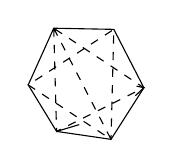
\begin{tikzpicture}[scale=.72]
\draw (-1,0)--(-.55,1)--(.51,.98)--(1.04,-.05)--(.46,-.96)--(-.5,-.82)--cycle;
\draw[dashed] (-.55,1)--(.46,-.96)--(-1,0)--(.51,.98)--(.46,-.96)
 (-.55,1)--(-.5,-.82)--(1.04,-.05)--(-.55,1);
\draw (-.5,-.82)--(-.10,-.7) (.91,-.02)--(1.04,-.05)--(.89,-.19);
\end{tikzpicture}}
% archive sheet number: 43
